\section{Theory}
\def \kapitelautor {Christoph Führer}
% TODO explain technical theory

\section{Technologies}
\def \kapitelautor {Christoph Führer}
% TODO explain used technologies

\section{Planning and Prototyping} % PoC
\def \kapitelautor {Erik Ritschl}

Our work already began in the summer of 2015. Since Python was a new language to all of us, and we had especially little experience with wxPython and GUI programming in general, we decided this was the best time to acquaint ourselves with these topics. So we read and watched many tutorials on the Internet, until we felt comfortable about carrying out a project with them.

A mini-prototype was also created, as a proof of concept. It had a very minimalistic graphical user interface, and was capable of the following:

\begin{itemize}
	\item Read tags from a database file
	\item Read relations between tags and files
	\item Create folders for tags
	\item Create symbolic links in these folders that point to the according file
\end{itemize}

In this phase, another feature was also planned, as a must-requirement even, that had to be dropped. The software was supposed to be able to save tags not only in the central database file, but also in the meta information of the file itself. Attempts have been made at implementing this functionality, first with EXIF, then IPTC and lastly XMP (all different kinds of meta data, where the first two only work with images and the last one with all files). But it quickly became evident during development of the prototype that there is no easy way to modify meta data with Python on all the platforms that we support (Windows, OS X and Ubuntu).
\paragraph{}
After the summer holidays had ended, the team sat together and decided upon the exact features the software should have. These were then formulated as user stories and together composed the product backlog. Soon after that, a method called \href{https://en.wikipedia.org/wiki/Planning_poker}{Planning Poker} was used in order to decide how many points each user story should be assigned. These points are used to describe the complexity of a user story, and help estimating the total time a task needs in order to be completed.

\paragraph{}
With the completion of the product backlog, the next logical step was to develop a paper prototype. A section of the frontend was assigned to each team member, who subsequently drew sketches with a pen and paper. These were then discussed with the team, and the process was repeated until everyone was happy with the end result.

% TODO: embed sketches, explain frontend


% TODO chronological order
% function prototypes, learning python
% product backlog
% planning poker
% paper prototype
% code snippets

\section{Structure}
\def \kapitelautor {Clemens Stadlbauer}

In our code repository there are several folders, each of which containing a
certain category of files.

\begin{itemize}
	\item[\tfpath{doc/}] The documentation of the software, i.e. the user manual
	\item[\tfpath{icons/}] All the different icons and the logo used throughout the
	software
	\item[\tfpath{db/}] Database schemas and the database setup script
	\item[\tfpath{src/}] The actual code of the software
\end{itemize}

\subsection{db}
In \tfpath{system.sql} is the schema of the main database. It contains the user
settings and the location of all the galleries. Every gallery has its own
database as described in \tfpath{gallery.sql} containing all imported files,
all created tags and all created output folders. The connections between these
items (for example which tags a files has) are recorded in addition,
intermediate tables.

Furthermore, the directory contains a helper script to create the initial
system database and an empty gallery database which is copied every time a new
gallery is created by the user.

\subsection{src}
Herein lie all the modules that make up the entirety of the functionality and
design of OctoTagger. Each module is contained in a single file with the
module's name and can be categorizes as either frontend or backend. All the
frontend modules provide some part of the user interface while all the backend
modules implement mostly all the functionality that happens in the background
(for example the management of files).

% TODO module tree?

\section{Frontend}
%\subsection{Modulename}
\def \kapitelautor {}

\subsubsection{Abstract}

\subsubsection{Attempts}

\subsubsection{Solution} % TODO better title

\section{Backend}
%\subsection{Modulename}
\def \kapitelautor {}

\subsubsection{Abstract}

\subsubsection{Attempts}

\subsubsection{Solution} % TODO better title

% TODO explain code
% each module has a small abstract explaining what and how it works
% each module explained roughly in chronological order

\section{Corporate Design}
%\subsection{Corporate Identity}

What is the first thing you should think about, when you see our logo? Why did we use these colors? Why did we decide to take this font? 

These are just a few questions related to the corporate identity. It determinates how the project team presents itself to the public. Within the corporate identity document everything regarding public appearance can be defined. This could contain the behaviour to the public, as well as communication, philosophy, design, language and much more. 

In case of OctoTagger it was decided to just take care of the design part from the corporate identity, the corporate design. This document contains our design-guidelines for the website. This includes the colors used for the logo and other images, the background colors, the font and the logo itself. 

The challenge at developing a corporate design is to always keep the user in mind. How does the user think? What does he want to see? It's important to attract a potential user and catch his attention. The website is the first thing every potential user gets confronted with, so it has to send the right signals. Colors are great triggers for emotions and feelings making them a powerful tool for the writer of the corporate design. However, the proper combination of the colors is at least as important as the colors themselves. 

The logo design should not be neglected. It's an essential part of the corporate design. The challenge is to design a logo that provides a distinctive look but keeping it as simple as possible at the same time. 

\subsection{Background of the name OctoTagger}

In the beginning there was just the idea for the product, an file organisation software. Afterwards the name OctoTagger was born. The intention behind that name was indeed an octopus and it's ability to handle several actions at the same time, due to his eight arms. In this point OctoTagger and octopuses share similarities. OctoTagger is also able to handle multiple files at the same time. So the octopus became our mascot and the corporate design was developed out of this idea later. 

\subsection{Corporate Design for OctoTagger}
\subsubsection{Colors}

The colors were the first part of the corporate design to be defined. Because of our mascot the octopus, it was decided to chose colors related to the living environment of octopuses which is the sea. We picked several shades of green and blue to fit this scheme. These tones became our primary colors which means that they are used most of the time. However, just using this colors would be too monotonous, so a secondary color set was added. It contains some complementary colors of the primary colors and is just used rarely.

\paragraph{Primary Colors} \hspace{0pt} \\

\definecolor{primary_1}{RGB}{118,178,76}
\definecolor{primary_2}{RGB}{49,201,175}
\definecolor{primary_5}{RGB}{130,227,166}
\definecolor{primary_3}{RGB}{23,197,200}
\definecolor{primary_6}{RGB}{123,215,213}
\definecolor{primary_4}{RGB}{59,177,216}

\begin{tabular}{ c  c  c  c }
\#76B24C & \crule[primary_1]{3cm}{3cm} & \#31C9AF & \crule[primary_2]{3cm}{3cm} \\
\#17BBC8 & \crule[primary_3]{3cm}{3cm} & \#3BB1D8 & \crule[primary_4]{3cm}{3cm} \\
\#82E3A6 & \crule[primary_5]{3cm}{3cm} & \#7BD7D5 & \crule[primary_6]{3cm}{3cm} \\ 
\end{tabular}

\paragraph{Secondary Colors} \hspace{0pt} \\

\definecolor{secondary_1}{RGB}{255,193,0}
\definecolor{secondary_2}{RGB}{255,140,62}
\definecolor{secondary_3}{RGB}{255,92,62}

\begin{tabular}{ c  c  c  c }
\#FFC100 & \crule[secondary_1]{3cm}{3cm} & \#FF8C3E & \crule[secondary_2]{3cm}{3cm} \\
\#FF5C3E & \crule[secondary_3]{3cm}{3cm} \\
\end{tabular}

\paragraph{Background Colors} \hspace{0pt} \\

\definecolor{background_1}{RGB}{240,240,240}
\definecolor{background_2}{RGB}{193,200,197}

\begin{tabular}{ c  c }
\#F0F0F0 & \crule[background_1]{6cm}{3cm} \\
\#C1C8C5 & \crule[background_2]{6cm}{3cm} \\
\end{tabular}\\



During the color-planing process it was decided to include two different background colors into the corporate design. The first one is a light gray shade which reduces the contrast between the background and the content above it. It is used as background color on the entire website. The second color consists of a much darker shade of gray. It's mainly used to create a second background layer over the first background. 

\subsubsection{Fonts}

As font, the DejaVu font family is used on the website. It follows the general guidelines of the OctoTagger website by being straight and modern. Below an example of the DejaVu font can be seen.\\

\begin{center}
	
\includegraphics[width=\linewidth]{images/font.png}
\end{center}

\subsubsection{Logo}

\paragraph{First drafts} \hspace{0pt} \\

The first concept for the logo of OctoTagger was the combination of an octopus and a folder symbol. These two elements were brought together seamlessly. However, it did not measure up to our expectations as the octopus was hardly recognizable. 

The sketch can be seen in the following image:

\begin{center}
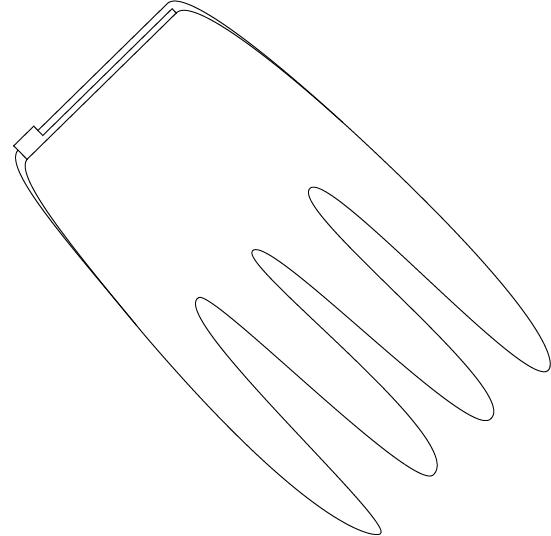
\includegraphics[scale=0.30]{images/logo_v01.png}
\end{center}

The second draft was an enhanced version of the first one. It was tried to keep it more even and linear, furthermore colors were added for the first time. This version of the logo consists of two parts, the file symbol on the top, symbolizing the body of the octopus, and four tentacles below it.

The image below shows the second sketch:

\begin{center}

\includegraphics[scale=0.30]{images/logo_v02.png}
\end{center}

This sketch became even more abstract then the first one and we got some negative feedback. Later it was replaced by an improved version, our actual logo.

\subsubsection{Current logo}

For the final version of the logo, the first concept was adopted and the idea of a folder symbol in our logo was dropped. It was decided to just include the octopus into the logo. This octopus has four visible tentacles on the front and four more in the background. At the end of these arms tags are attached.

The outcome can be seen below:


\begin{center}

\includegraphics[width=0.5\linewidth]{images/logo.png}

A version including the project name is also available:

\includegraphics[width=\linewidth]{images/logo_text.png}
\end{center}
% TODO message -> colors
\section{Website}
%\subsection{Why is a website important?}

A website is the most efficient way to represent the product as well as the project team. In case of OctoTagger the website also fulfils the task to distribute the product by offering a download. As web developer it's necessary to keep the target audience in mind and adjust the website to its needs.

\subsection{Concept of OctoTagger website}

The website of OctoTagger follows simple and decent design guidelines. It was designed to satisfy the users needs and being as lightweight as possible at the same time. Only few and small images are used on the entire site keeping loading times short.

A major aspect of the website is the ultra-lightweight, straight and modern design. The image design was kept clear and simple without the use of explicit borders. Due to that images appear flat and homogeneous.

\subsubsection{Usability}

The site was developed to be intuitive and easy to use. The user can reach every page independent of his current position.

To make navigation easier, clickable items were made as distinctive as possible. Only buttons and elements of the navigation bar respond to mouse clicks. These objects are also the only ones to respond to hovering, so the user gets signalled that after a click an action will be performed.

As an example for usability, downloading Octotagger could hardly be easier. Every button leading to a download, is colored in a shade of green, compared to other buttons colored in a shade of blue. In fact the user just has to click every green button, follow some installation instructions and is able to use Octotagger after a few minutes.

\subsubsection{Responsive Design}

The challenge for web development is to create a website, that looks good on every available screen size and device like desktop PCs, tablets, phablets and mobile phones. This can be ensured through different solutions.

The first option is to write different CSS sheets for every screen size or device, which requires the most work.

An easier possibility is called responsive design and there are numerous frameworks to support the developer with it. 

Responsive design means that a website is created to work on every device and adapts its appearance based on the screen size and orientation. The concept is based on flexible grids and layouts and the use of CSS media queries.

The following images show the OctoTagger website adapted to different screen sizes:

\begin{center}
\begin{tabular}{ c  c c }
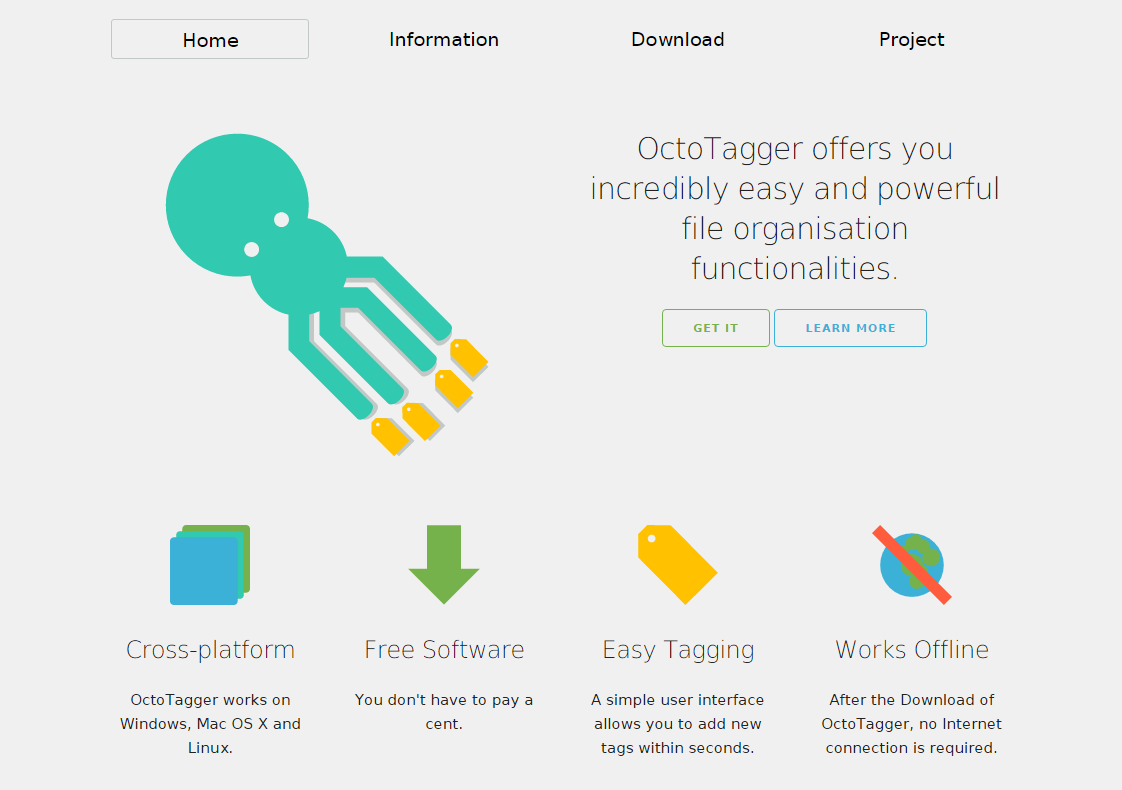
\includegraphics[scale=0.20]{images/home_full.png} & 
\includegraphics[scale=0.30]{images/resize.png} & 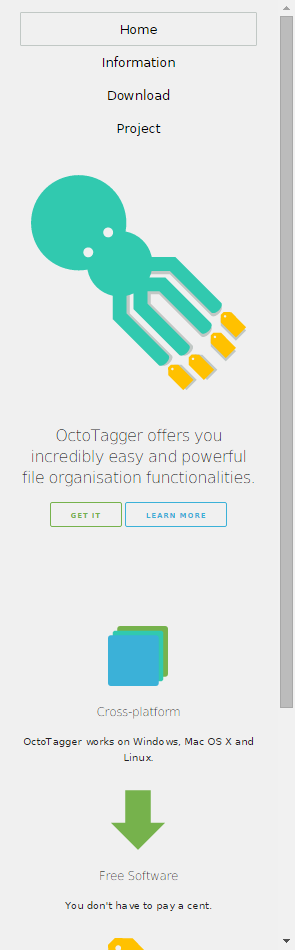
\includegraphics[scale=0.30]{images/home_small.png} \\
\end{tabular}
\end{center}

When the website passes a threshold during the resize, the elements are positioned above each other to fit the smaller screen width. The framework (see \ref{sec:Skeleton}) stacked the elements automatically, but adjustments were still necessary. Some media queries (see \ref{sec:MediaQueries}) had to be adapted so that elements fit perfectly together.

\paragraph{Flexible Grid} \hspace{0pt} \\

Most responsive framework rely on a flexible grid system, with typically 12 columns. Elements in the HTML code can now be positioned within this grid with the help of CSS classes. Depending on the width you want a HTML object to have, you have to give the proper CSS classes.

The image below shows a flexible grid example using the Skeleton framework (see \ref{sec:Skeleton})

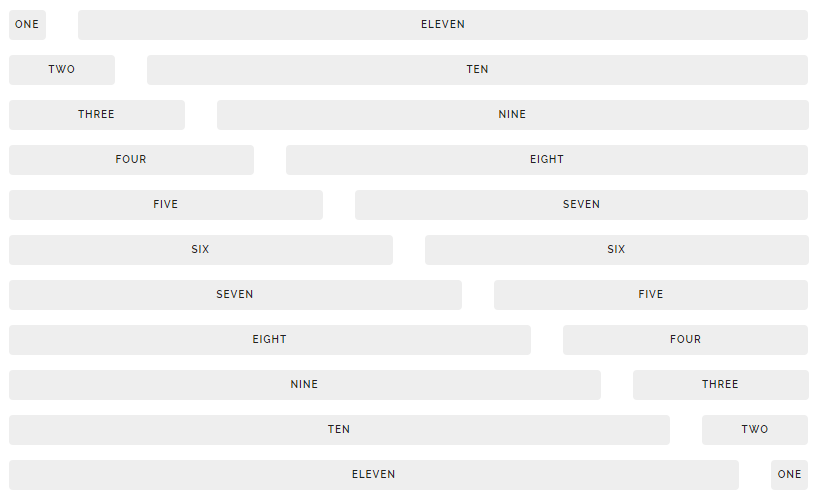
\includegraphics[scale=0.50]{images/skeleton_grid.png} 

\paragraph{CSS Media Queries} \hspace{0pt} \\
\label{sec:MediaQueries}

With the help of CSS Media Queries it's possible to set CSS attributes depending on conditions like screen width and device type. For instance the width of a box can  be increased when the window is enlarged.

The following code snippet shows an example for some width dependant media queries.

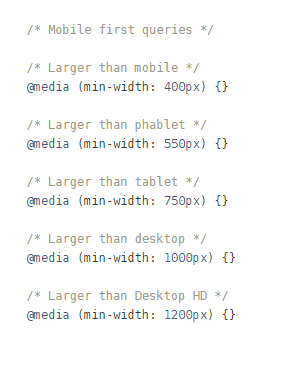
\includegraphics[scale=0.70]{images/media_query.png} 

\subsection{Structure}

The OctoTagger website is basically made up of four pages called Home, Information, Download and Project. All these pages are accessible via the navigation bar which is positioned on the top on every page. In addition there are several sub-pages only accessible on the download site.

\subsubsection{Home page}

\begin{center}
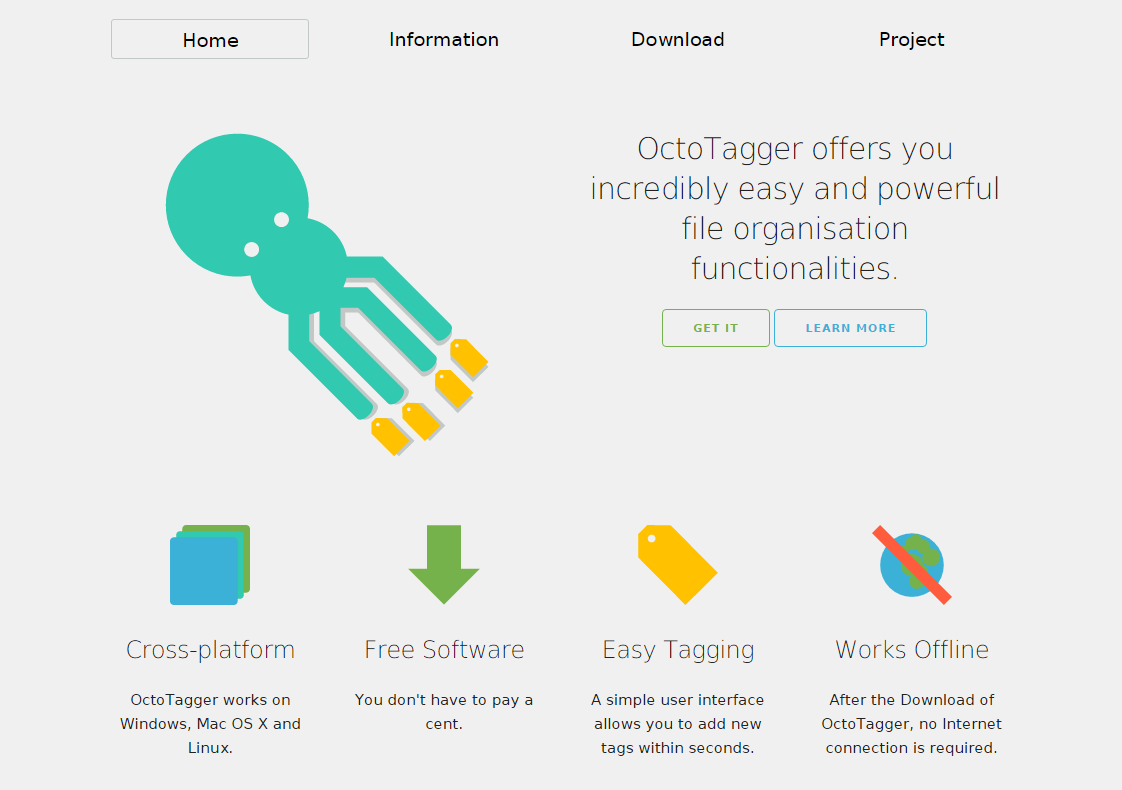
\includegraphics[scale=0.35]{images/home_full.png}\\
\end{center}

The home page is the first thing a user sees when he visits octotagger.co. This page is designed to catch the users attention with the help of a catchy slogan. The button "Learn more" is linked to the information page and with the help of the button "Get it" the user gets transferred to the download page. By just hovering the "Get it" button, a drop down menu appears and offers the possibility to directly download OctoTagger for the users operating system (see \ref{sec:OSdetection}). This option just makes sense, when the user has already installed the required software, of course.

In the bottom part the highlights of the software are pointed out with pictograms and short descriptions. The goal is to show the user the advantages of the software in one glance.

\subsubsection{Information page}

\begin{center}
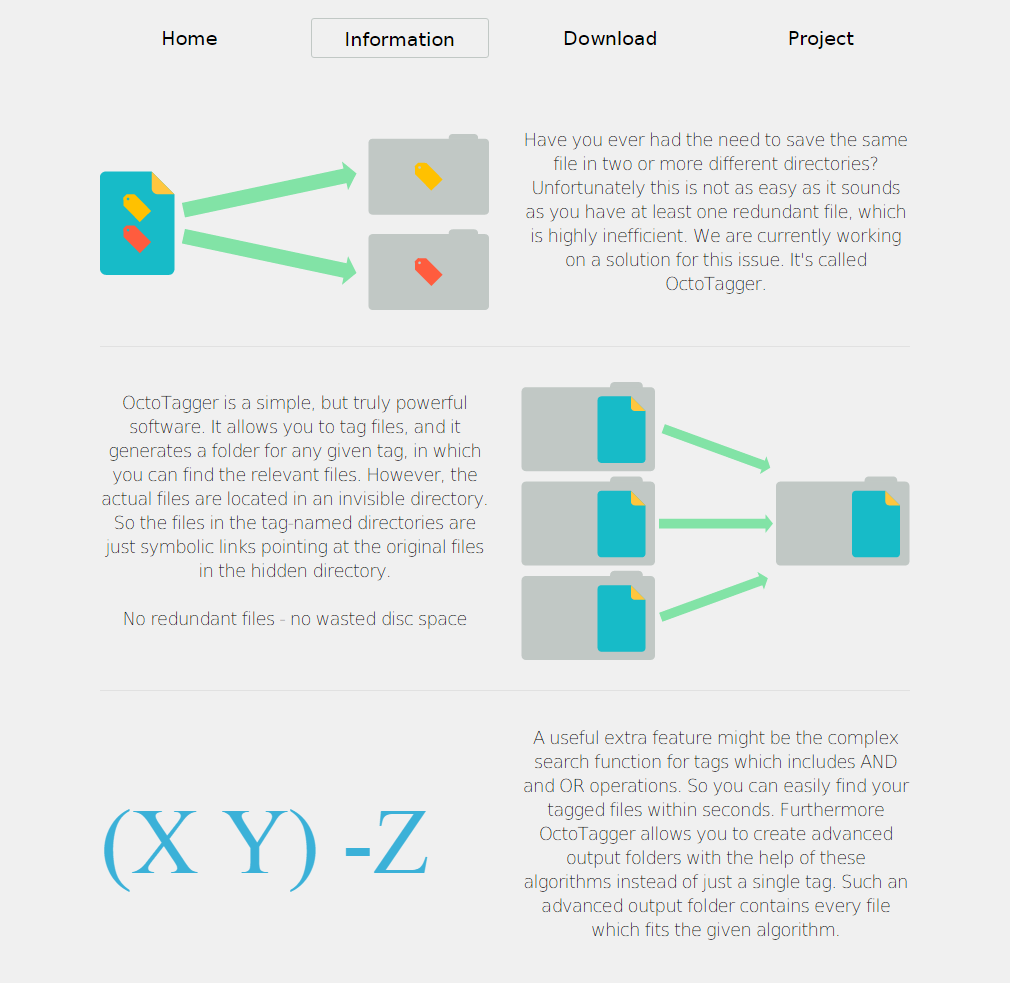
\includegraphics[scale=0.35]{images/information_full.png}
\end{center}

The information page offers the user some basic information about the functionality of OctoTagger. For this purpose, some simple images with short explanation text is shown. There is no previous knowledge needed to understand the explanation and the user doesn't have to deal with technical details.

\subsubsection{Download page}

\begin{center}
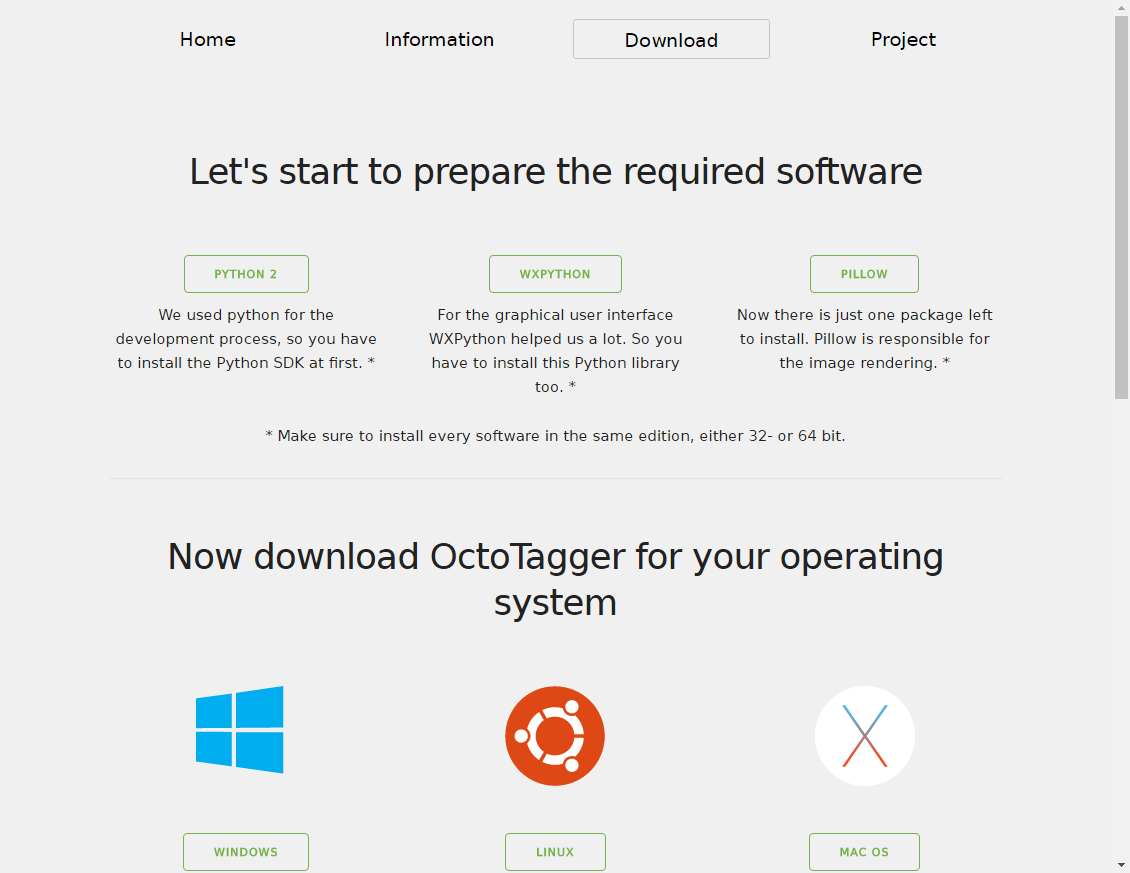
\includegraphics[scale=0.35]{images/download_full.png}
\end{center}

This page contains every available download and instructions for the installation. It's built like a step by step tutorial to guide the user through the entire process.

At first the user has to install the required software. The buttons on the top link to the developer website of the software. When a button is hovered, a dropdown menu shows up and offers further information. When the button is clicked the download site opens in a new tab.
 
The second step describes the installation of OctoTagger itself. These download buttons also provide hover functionality, which offers links to the installation guide. By clicking the download button the download starts directly. Windows user also have to install additional software to be able to use OctoTagger, which is described in the installation guide. 

In addition the user also has the possibility to download only Pywinlink, which is a service allowing symbolic links without the need of administrator rights. This service is required for OctoTagger on Windows, but is already included into the download above.

In the last step the user can download the user manual as PDF.

On the bottom of the page a link to the project Git repository can also be found.

\subsubsection{Project page}

\begin{center}
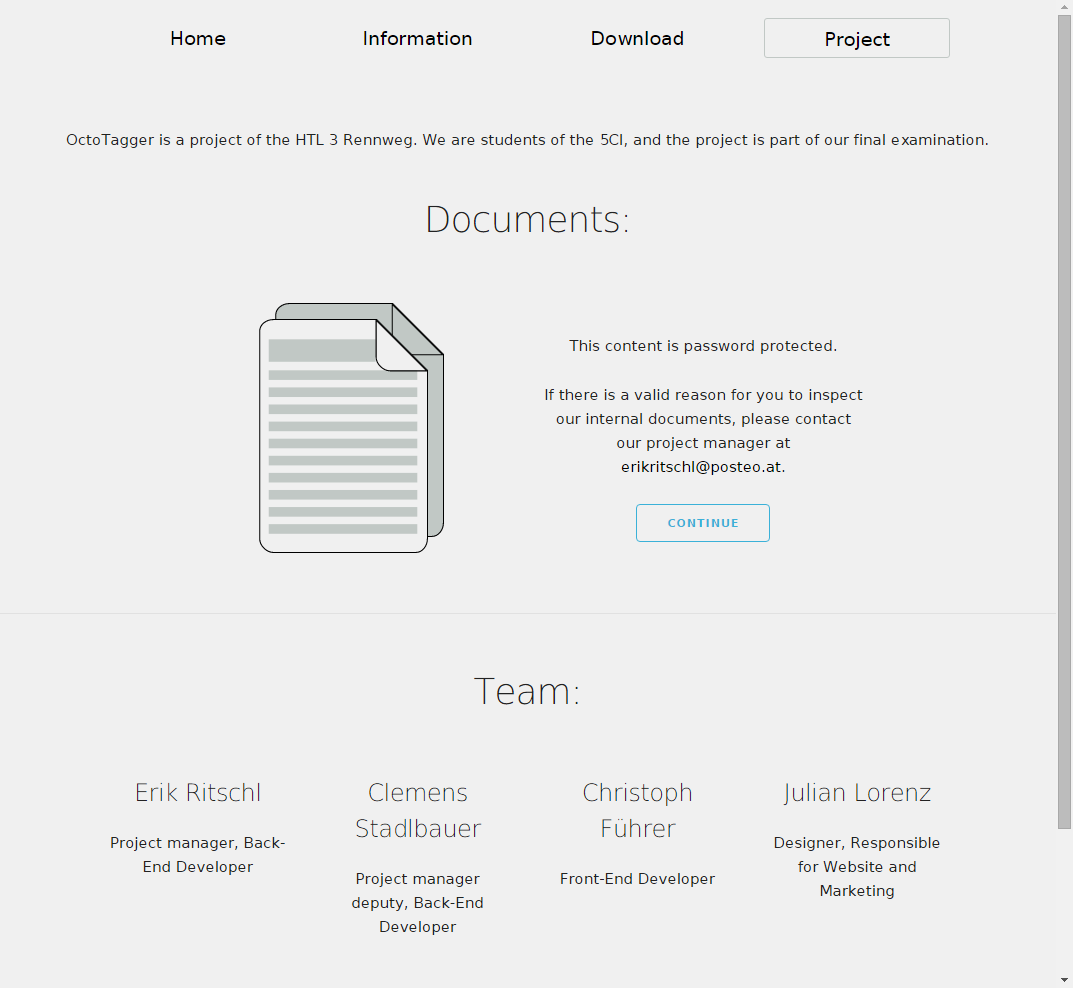
\includegraphics[scale=0.35]{images/project_full.png}
\end{center}

On this page information about the team, contact details and a link to some of our internal documents are brought together. 

\subsection{Used Tools and Technologies}

The following software, tools and frameworks helped us a lot at developing the website. Large and complex frameworks have completely been avoided to reduce loading times.


\subsubsection{Skeleton (Responsive CSS Framework)}
\label{sec:Skeleton}

Skeleton (http://getskeleton.com) is a framework which supports you with responsive development. Its source code consists of extremely few lines of code, making it great for small websites. Because of that Skeleton requires a lot of work of the developer and is basically only capable of managing the responsive grid system. It's everything you would need for responsive design, but nothing more.

\subsubsection{Adobe Illustrator}

This vector graphics editor was used for the creation of the images. 

\subsubsection{Sublime Text (Editor)}

\subsubsection{Operation System detection}
\label{sec:OSdetection}

Javascript allows the developer to check the user's operating system within just one line of code.



\subsection{Hosting}

The server is operated by the cloud provider Cloudatcost. This provider was chosen due to positive experiences in past projects and the possibility to buy a server for all time by a one-time payment. In addition, the price of 35 \$ for a simple web server is affordable for our project team. 

The server provides more then enough processing power for our needs and it's possible to install every available software on it thanks to command line control.

Namecheap was our choice concerning the purchase of the domain. This made another 8.88 \$ to use octotagger.co for one year.
% TODO like module

\section{Quality Management}
\def \kapitelautor {Julian Lorenz}
% TODO
